\documentclass[a4paper,10pt]{article}
\usepackage[utf8]{inputenc}
\usepackage{comment}

\usepackage[
backend=biber,
style=alphabetic,
sorting=ynt
]{biblatex}
\addbibresource{bibliography.bib}   %>>>> bibliography data in bibliography.bib
%\bibliography{bibliography}   %>>>> bibliography data in bibliography.bib
%\bibliographystyle{spiebib}   %>>>> makes bibtex use spiebib.bst


%%%%%%%%%%%%%%%%%%%%%%%%%%%%%%%%%%%%%%%%%%%%%%%%%%%%%%%%%%%%%%%%%%%%%%%%%%%%%%%%
\usepackage{url}
%
\usepackage[breaklinks]{hyperref}
\usepackage{breakurl}

%%%%%%%%%%%%%%%%%%%%%%%%%%%%%%%%%%%%%%%%%%%%%%%%%%%%%%%%%%%%%%%%%%%%%%%%%%%%%%%%
\usepackage{graphicx}
\usepackage{subcaption}
%%%%%%%%%%%%%%%%%%%%%%%%%%%%%%%%%%%%%%%%%%%%%%%%%%%%%%%%%%%%%%%%%%%%%%%%%%%%%%%%

\usepackage[svgnames]{xcolor} % Enabling colors by their 'svgnames'

\usepackage{amsmath}
\usepackage{amsfonts}
\usepackage{amssymb}


%%%%%%%%%%%%%%%%%%%%%%%%%%%%%%%%%%%%%%%%%%%%%%%%%%%%%%%%%%%%%%%%%%%%%%%%%%%%%%%%
\usepackage{amsthm}
\newtheorem{mydef}{Definição}

%%%%%%%%%%%%%%%%%%%%%%%%%%%%%%%%%%%%%%%%%%%%%%%%%%%%%%%%%%%%%%%%%%%%%%%%%%%%%%%%

%opening
\title{Dança, Canais de Comunicação e Condução Compartilhada}
\author{Fernando Pujaico Rivera}

%%%%%%%%%%%%%%%%%%%%%%%%%%%%%%%%%%%%%%%%%%%%%%%%%%%%%%%%%%%%%%%%%%%%%%%%%%%%%%%%
%%%%%%%%%%%%%%%%%%%%%%%%%%%%%%%%%%%%%%%%%%%%%%%%%%%%%%%%%%%%%%%%%%%%%%%%%%%%%%%%
%%%%%%%%%%%%%%%%%%%%%%%%%%%%%%%%%%%%%%%%%%%%%%%%%%%%%%%%%%%%%%%%%%%%%%%%%%%%%%%%
%%%%%%%%%%%%%%%%%%%%%%%%%%%%%%%%%%%%%%%%%%%%%%%%%%%%%%%%%%%%%%%%%%%%%%%%%%%%%%%%
\begin{document}

\maketitle

\begin{abstract}
Condução compartilhada
\end{abstract}
\section{Definições}

\begin{mydef}[Paradigma]
Algo que serve de exemplo ou modelo; padrão \cite{michaelis.uol.com.br}.
\end{mydef}

\begin{mydef}[Condutor]
Definiremos aqui, condutor como a pessoa encarregada de propôr um movimento, passo ou ação na dança a dóis.
Esta proposta pode ser feita de maneira indicativa, corporal, por indução ou por ausência.
\end{mydef}

\begin{mydef}[Seguidor]
Definiremos aqui, seguidor como a pessoa encarregada de  receber a proposta de movimento, passo ou ação  na dança a dóis,
e realizar uma resposta corporal a esta.
A proposta pode chegar de maneira indicativa, corporal, por indução ou por ausência.
\end{mydef}

\begin{mydef}[Paradigma da condução]
Definiremos aqui, o paradigma da condução ou simplesmente condução, como o modelo de dança a dóis no qual a informação da proposta do movimento, 
passo ou ação é transmitida unidirecionalmente, 
desde um condutor ate um seguidor.
Neste modelo de dança o papel do condutor e do seguidor é fixo.


Os autores Maia, M.A.C. e Pereira, V.R. \cite{maia2010danca} explicam que 
essa transmissão de informação acontece por médio dos pontos onde há contato corporal, numa troca de energia constante,
sendo o contato e o adecuado nível de pressão importantes para ser bons condutores e seguidores.

Por outro lado, autores como Feitosa J. K. se questiona na suas pesquisas \cite[pp. 24]{Jonas2011},
se o papel do seguidor deve ser apenas resistir à condução do condutor e produzir o charme na dança?
Motivando assim a procura e proposta outros paradigmas na dança a dois.

\end{mydef}

\section{Modos de operação de um canal de comunicação}

Podemos estabelecer uma canal de comunicação baixo distintos modos de operação, 
entre estes modos temos o ``Simplex channel'', o ``Half duplex channel'' e o 
``Duplex channel'' \cite[pp.60 ]{hura2001data}\cite[pp. 5]{shinde2009computer}.

O \textbf{Simplex channel} denota um médio de comunicação habilitado 
para transmitir dados unicamente numa direção, desde o transmissor ate o receptor 
sendo que estes papeis são designados de maneira fixa 
\cite[pp. 5]{shinde2009computer} \cite[pp. 430]{sawaya2002dicionario} \cite[pp.60 ]{hura2001data}, 
um exemplo disto pode ser visto num sistema de transmissão de rádio onde a emissora 
transmite a música, e o usuário está habilitado só pra receber os dados e escutar, 
ver Figura \ref{fig:channelsimplex}. 

O \textbf{Half duplex channel} denota um médio de comunicação onde o canal está
sendo usado em uma direção por vez, 
porem esta direção cambia de modo que os papeis de transmissor e receptor são 
intercambiáveis entre os usuários 
\cite[pp. 5]{shinde2009computer}\cite[pp. 208]{sawaya2002dicionario}. 
Neste modo de comunicação o fim da mensagem em uma direção é 
reconhecida pelo receptor que pode cambiar a direção do modo de transmissão,
geralmente existe um tempo de pausa para esperar a troca de emissor se esta existir \cite[pp. 60]{hura2001data}.
ver Figura \ref{fig:channelhalfduplex}. 

O \textbf{Full duplex channel} ou  \textbf{Duplex channel} denota um médio de comunicação onde o
canal permite a transmissão simultânea em ambas as direções \cite[pp. 150]{sawaya2002dicionario},
de modo que no existe o tempo de pausa para a troca do sentido da transmissão como nos canais ``Half duplex'' \cite[pp. 5]{shinde2009computer},
este método de comunicação pode ser implementado fusionando dois ``simplex channel'' \cite[pp. 60]{hura2001data}.
\begin{figure}[ht!]
    \centering
    \begin{subfigure}[b]{0.3\textwidth}
        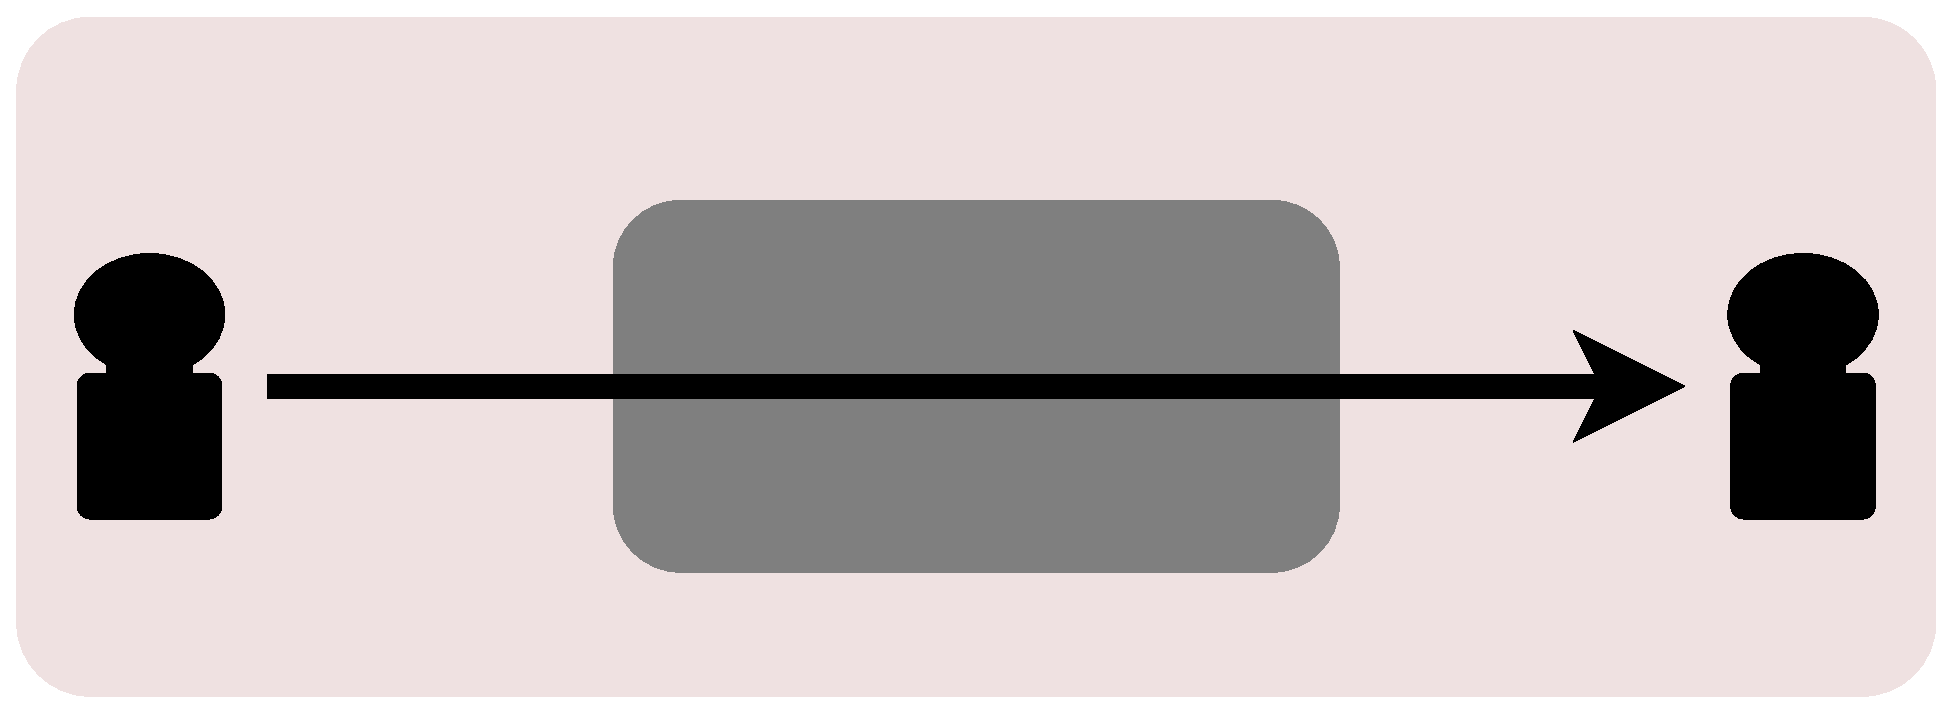
\includegraphics[width=\textwidth]{channel-simplex.eps}
        \caption{Simplex channel}
        \label{fig:channelsimplex}
    \end{subfigure}
    ~ %add desired spacing between images, e. g. ~, \quad, \qquad, \hfill etc. 
      %(or a blank line to force the subfigure onto a new line)
    \begin{subfigure}[b]{0.3\textwidth}
        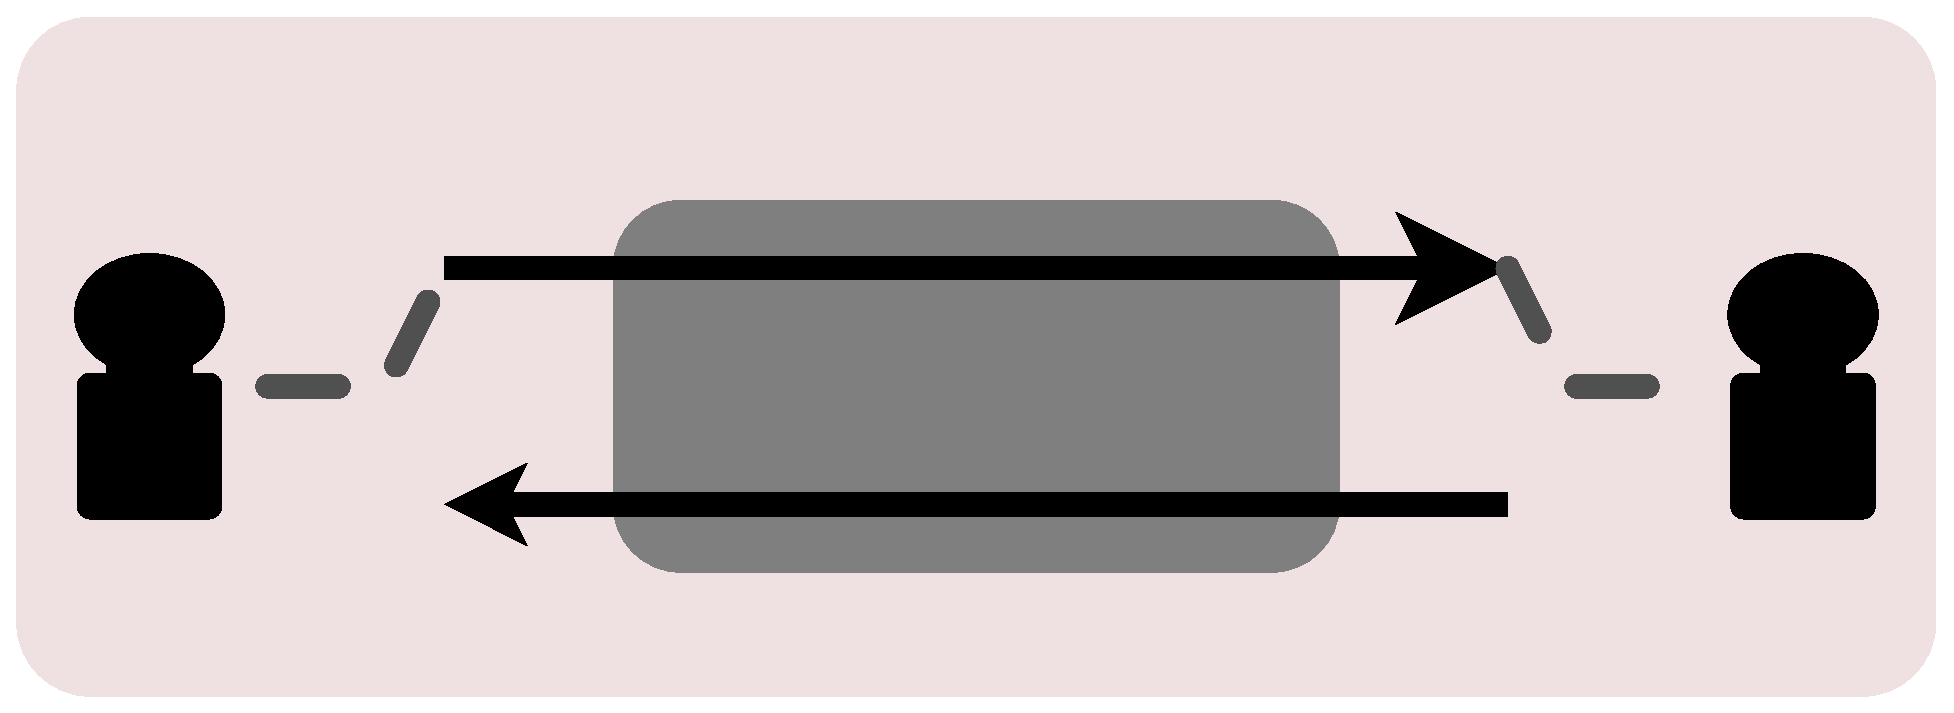
\includegraphics[width=\textwidth]{channel-halfduplex.eps}
        \caption{Half duplex channel}
        \label{fig:channelhalfduplex}
    \end{subfigure}
    ~ %add desired spacing between images, e. g. ~, \quad, \qquad, \hfill etc. 
    %(or a blank line to force the subfigure onto a new line)
    \begin{subfigure}[b]{0.3\textwidth}
        \includegraphics[width=\textwidth]{channel-duplex.eps}
        \caption{Duplex channel}
        \label{fig:channelduplex}
    \end{subfigure}
    \caption{Modos de operação}\label{fig:channeltypes}
\end{figure}


\section{Paradigma na dança vs. Modos de transmissão}

\begin{table}[h!]
  \begin{center}
    \caption{Your first table.}
    \label{tab:table1}
    \begin{tabular}{|l|c|r|} % ff
    \hline
      Modos de transmissão & Paradigma \\ \hline \hline
      Simplex channel & Condução  \\ \hline
      Half duplex channel & Condução com troca de condutor \\ \hline
      Duplex channel & Condução compartilhada \\ \hline
    \end{tabular}
  \end{center}
\end{table}


\section{Conclusões}
Nas minhas pesquisas sobre dança compartilhada, 
tenho achado muito material não 
acadêmico\footnote{Postagens em blogs com temas relativos a dança.} 
focando a importância deste paradigma na dança, 
numa luta social sobre o papel das pessoas na dança seguindo o sexo.
Acho que é um error promover ou divulgar a dança compartilhada 
como um método para a liberação da opressão do condutor escolhido por seu sexo, 
isso só é uma postura ideológica. 
Se só isso fosse o problema, 
bastaria com empoderar as pessoas que atualmente não usam, 
ou se planteiam usar, esse papel na sociedade, 
a tomar ou pedir o papel de condutor nas danças, 
dado que não existe nenhuma norma que o proíba  
ou que exija em caráter mandatório o papel de um individuo na condução seguindo o sexo,
isso ate agora era só uma convenção social, 
dado que o único método de comunicação conhecido na dança era a comunicação unidirecional de emissor fixo,
e consequentemente um individuo devia tomar o papel de condutor e outro de seguidor. 
Assim, neste enfoque o papel de condutor está habilitado para toda pessoa que se interesse em 
cultivarlo e aprenderlo. 
Pelo qual se promovemos o valor da dança compartilhada nesse aspecto, 
esta não teria sentido de existir, 
pois nenhuma pessoa está proibida de tomar este papel.

Por outo lado, a um nível técnico e fácil perceber que na dança, além da comunicação 
unidirecional de emissor fixo  (paradigma da condução),
existem alguns outros modos de comunicação pouco explorados ate agora,
como a comunicação com troca de emissor, 
usando o canal de transmissão em um sentido por vez,
e também a comunicação bidirecional com mensagens indo de um lado a outro em simultâneo.
Ate agora a porta do conhecimento e pesquisa estava unicamente aberta para a 
comunicação unidirecional de emissor fixo, 
sendo que as outras duas portas restantes antes mencionadas estão ainda pouco 
exploradas e com infinitas possibilidades a descobrir e pesquisar; 
na minha humilde opinião, este é o verdadeiro valor da dança compartilhada. 

%%%%%%%%%%%%%%%%%%%%%%%%%%%%%%%%%%%%%%%%%%%%%%%%%%%%%%%%%%%%%%%%%%%%%%%%%%%%%%%%
%%%%%%%%%%%%%%%%%%%%%%%%%%%%%%%%%%%%%%%%%%%%%%%%%%%%%%%%%%%%%%%%%%%%%%%%%%%%%%%%
%%%%%%%%%%%%%%%%%%%%%%%%%%%%%%%%%%%%%%%%%%%%%%%%%%%%%%%%%%%%%%%%%%%%%%%%%%%%%%%%
%%%%%%%%%%%%%%%%%%%%%%%%%%%%%%%%%%%%%%%%%%%%%%%%%%%%%%%%%%%%%%%%%%%%%%%%%%%%%%%%

\medskip
 
\printbibliography

\end{document}
